\documentclass[10pt,fleqn, % linksbündige, abgesetzte Formeln% ===> this file was generated automatically by noweave --- better not edit it
reqno,a4paper]{article}
\usepackage[utf8]{inputenc}
\usepackage{amsfonts}
%\usepackage{ngerman}
\usepackage[german, english]{babel}
\usepackage{graphicx}
\usepackage{caption}
\usepackage{subcaption}
\usepackage[hidelinks]{hyperref}
\usepackage[square,sort,comma,numbers]{natbib}% bibliography style for support for urls in the bibliography
\usepackage{noweb}
\pagestyle{plain}% plain without headlines, with something more \pagestyle{noweb}
\noweboptions{shift,smallcode,longchunks}%german,smallcode,longchunks
\usepackage[dvipsnames]{xcolor}
\usepackage{comment}
\usepackage{geometry}
\usepackage{tikz}
\geometry{a4paper, portrait,left=2.5cm, right=2.5cm, top=2cm, bottom=2cm}
\usepackage[T1]{fontenc}
\usepackage[tbtags, % Platzierung der Formel-Tags;% es gibt auch centertags
sumlimits,
% Platzierung der Summationsgrenzen
% (oberhalb/unterhalb)
intlimits,
% Platzierung der Integrationsgrenzen
% (oberhalb/unterhalb)
namelimits]
% Platzierung der Grenzen
% (oberhalb/unterhalb) bei Funktionen
{amsmath}

\usepackage{icomma}% für die richtige Kommadarstellung in Formeln und in Texten
\usepackage[toc,page]{appendix}
\usepackage{listings}% TXT Dateien in LaTeX einbinden

% Farbige Formeln richtig einfärben über die group Umgebung
\def\mathcolor#1#{\@mathcolor{#1}}
\def\@mathcolor#1#2#3{%
        \protect\leavevmode
        \begingroup\color#1{#2}#3\endgroup
}
%\newcommand{\na}{\mathcolor{blue!50!black}{a}}
\newcommand{\nx}{\mathcolor{gray}{x}}
\newcommand{\nX}{\mathcolor{gray}{X}}
\newcommand{\nnx}{\mathcolor{green!50!black}{x}}
%\newcommand{\nx}{\mathcolor{cyan!70!black}{x}}
\newcommand{\ny}{\mathcolor{gray}{y}}
%\newcommand{\nz}{\mathcolor{green!30!black}{\textit{z}}}
%\newcommand{\nA}{\mathcolor{green!50!black}{A}}
\newcommand{\nw}{\mathcolor{gray}{w}}
%\newcommand{\nW}{\mathcolor{gray}{W}}
\newcommand{\nt}{\mathcolor{gray}{t}}
\newcommand{\ntau}{\mathcolor{gray}{\tau}}
\newcommand{\nW}{\mathcolor{brown!70!black}{W}}
\newcommand{\neta}{\mathcolor{cyan!70!black}{\eta}}
\newcommand{\nnu}{\mathcolor{cyan!70!black}{u}}
\newcommand{\nnv}{\mathcolor{cyan!70!black}{v}}
\newcommand{\nsin}{\mathcolor{blue!70!black}{\sin}}
\newcommand{\ncos}{\mathcolor{blue!70!black}{\cos}}
\newcommand{\ntan}{\mathcolor{blue!70!black}{\tan}}
\newcommand{\narctan}{\mathcolor{blue!70!black}{\arctan}}
\newcommand{\ncosh}{\mathcolor{blue!70!black}{\cosh}}
\newcommand{\nsinh}{\mathcolor{blue!70!black}{\sinh}}
\newcommand{\nexp}{\mathcolor{blue!70!black}{\exp}}
\newcommand{\nf}{\mathcolor{blue!70!black}{f}}
\newcommand{\nni}{\mathcolor{red!70!black}{i}}
\newcommand{\nm}{\mathcolor{red!70!black}{m}}
\newcommand{\nn}{\mathcolor{red!70!black}{n}}
\newcommand{\nk}{\mathcolor{red!70!black}{k}}
\newcommand{\nl}{\mathcolor{red!70!black}{l}}
\newcommand{\nq}{\mathcolor{red!70!black}{q}}
\newcommand{\nh}{\mathcolor{blue!70!black}{h}}
\newcommand{\nA}{\mathcolor{blue!70!black}{A}}
\newcommand{\nV}{\mathcolor{blue!70!black}{V}}
\newcommand{\nxi}{\mathcolor{blue!70!black}{\xi}}
\newcommand{\dif}{\mathrm{\mathcolor{blue!70!black}{d } } }
\newcommand{\ndelta}{\mathcolor{blue!70!black}{\delta}}
\newcommand{\na}{\mathcolor{blue!70!black}{a}}
\newcommand{\nb}{\mathcolor{blue!70!black}{b}}
\newcommand{\nN}{\mathcolor{blue!70!black}{N}}
\newcommand{\nphi}{\mathcolor{blue!70!black}{\phi}}
\newcommand{\nr}{\mathcolor{blue!70!black}{r}}
\newcommand{\nT}{\mathcolor{blue!70!black}{T}}
\newcommand{\nln}{\mathcolor{blue!70!black}{\ln}}
\newcommand{\nD}{\mathcolor{green!50!black}{D}}
\newcommand{\nz}{\mathcolor{brown!70!black}{z}}
\newcommand{\nF}{\mathcolor{blue!70!black}{F}}
\newcommand{\mA}{\mathcolor{green!50!black}{A}}
\newcommand{\nC}{\mathcolor{cyan!70!black}{C}}
\newcommand{\npartial}{\mathcolor{blue!70!black}{\partial}}

\begin{document}\selectlanguage{english}
\begin{titlepage}

\begin{center}


% Oberer Teil der Titelseite:

\begin{minipage}{0.57\textwidth}
\begin{flushleft}\large
\begin{center}
Universität Potsdam\\
Mathematisch-Naturwisssenschaftliche Fakultät\\
Institut für Physik und Astronomie\\
\end{center}
\end{flushleft}
\end{minipage}
\hfill
\begin{minipage}{0.42\textwidth}
\begin{flushright}
\begin{center}

\includegraphics[width=0.55\textwidth]{logo.png}\\ 
\end{center}
\end{flushright}
\end{minipage}
\vfill
\vspace*{0.5cm}
\textsc{\large Computational Physics}\\[0.5cm]


% Title
%\newcommand{\HRule}{\rule{\linewidth}{0.5mm}}
%\HRule \\[0.4cm]
{ \Huge \bfseries Falling liquid films \\
Kuramoto-Sivashinsky equation}\\[0.4cm]

%\HRule \\[1.5cm]
\vspace*{2.5cm}

% Author and supervisor
\begin{minipage}{0.45\textwidth}
\begin{flushleft} \normalsize 
Author: Christian Gößl\\
Matrikel-No.:762627

\end{flushleft}
\end{minipage}
\hfill
\begin{minipage}{0.45\textwidth}
\begin{flushright} \normalsize 
\begin{flushleft}
corrector: Prof. Dr.~Arkady Pikovsky\\
\end{flushleft}
\end{flushright}
\end{minipage}

\vfill
{\normalsize  \today}
\vspace*{4.5cm}
% Unterer Teil der Seite


\end{center}

\end{titlepage}
\tableofcontents
\newpage

\nwfilename{falling-liquid-films.nw}\nwbegindocs{1}\nwdocspar
\begin{comment}


@language patch
Protocol

\begin{verbatim}

*****understanding
+  (1) derivation of the parameter equation

***** protocoll
-  control everywhere the correct time form of the verbs
-  read through the whole document

+  w introduction
+  w theory
+     w (1)
+     w (2)
+     w (3)
+     w (4)
+        w (4.1)
+        w (4.2)
+        w (4.3)
+     w numerical method
+  w c simulation
+     c plots
+     w docu
+        w stable
+        w turbulent
+        w coefficients
+  w conclusion
+  w c sources
+  w code documentation

\end{verbatim}
@language latex
\newpage

\end{comment}

\section{Introduction}
On a heavy raining day you see, that water is flowing down the window.
There you can find also some small waves, they are going down. 
In order to describe this phenomenon, physicists used a plait and investigated the water flow on that.
Usually, in our everyday life the window is perpendicular to the ground.
They changed the angle to ground from 90 to 0 degrees. 
In that arrangement the flow depends on the angle and they find formulas to describe the behavior of the flow.  
The falling liquid films produces wavetrains see figure \ref{pic:fastwave}.
They found, that the flowing can be turbulent see figure \ref{pic:downstream}.   


\begin{figure}[htp!]
        \begin{center}
                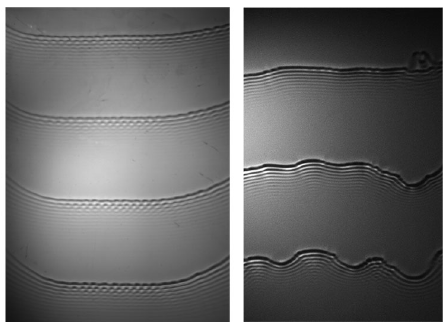
\includegraphics[scale=0.7]{secondary-3d-instabilities.png}
                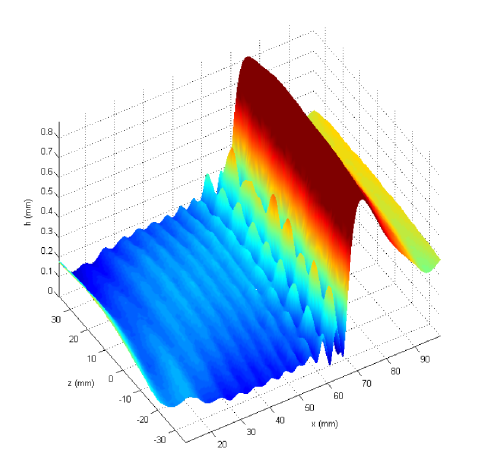
\includegraphics[scale=0.5]{modulated-fast-wave.png}
        \end{center}
        \caption{The left picture shows falling liquid films of physical experiment. The wave trains are going down and creating some nonregular structures.\cite{miyara_numerical_2000} The right picture shows a simulation of the falling liquid film wave trains in 3D. \cite{ruyer-quil_dynamics_2014}}
        \label{pic:fastwave}
\end{figure}

\begin{figure}[htp!]
        \begin{center}
                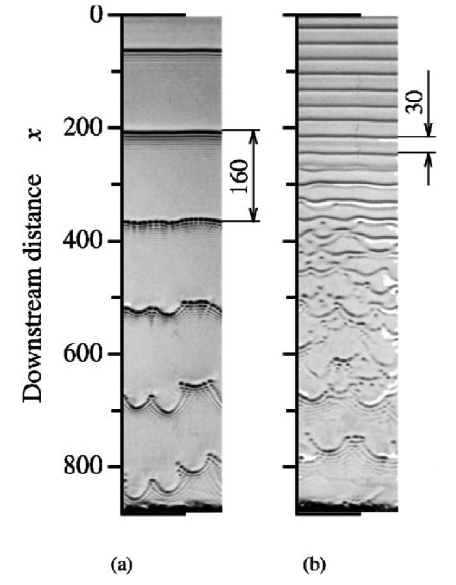
\includegraphics[scale=0.7]{downstream-23-degree.png}
        \end{center}
\caption{The falling liquid films producing waves. When the distance is growing the waves are transformed to a more unregular wave patterns, then we have a turbulent flow. \cite{miyara_numerical_2000}}
        \label{pic:downstream}
\end{figure}

In that work we want to simulate those turbulent flows. For that purpose we used a 1D formulation of that problem, the Kuramoto-Sivashinsky equation. We will investigate, which parameters are important for producing turbulence and how the turbulent flow will appear. 

\newpage

\section{Theory}
In that work, we want to simulate falling liquid films on a plaid. 
There we can find turbulent solution.
Usually, it is described in two or three dimensions, we took the one dimensional approach to show the turbulent behavior of the fluid at a specific choice of values of physical parameters. 
We describe the physical phenomenon with the typical variables: $ \nt $, $ \nx $ and $ \nnu $, displacement, time and velocity. The width is $ L $. We used the Kuramoto-Sivashinsky equation, which was derived by Yoshiki Kuramoto and Takeo Tsuzuki \cite{kuramoto_persistent_1976} and by Gregory Sivashinsky \cite{sivashinsky_nonlinear_1988}, here in a general form: 
\begin{align}
        a\frac{\npartial \nnu}{\npartial \nt} + b\frac{1}{2}\frac{\npartial (\nnu ^2) }{\npartial \nx} +c\frac{\npartial^2 \nnu}{\npartial \nx^2} +d\frac{\npartial^4 \nnu}{\npartial \nx^4} = 0  \label{eq:gen}
\end{align}
We rescale the equation in the variables $ \nt $, $ \nx $ and $ \nnu $.
We take for $ \nnu $ and $ \nx $ the transformation as follows
\begin{align*}
        \nx = \frac{\ny}{b} \quad \npartial_{\nx} = b \npartial_{\nx} \quad \nnu = \frac{\nnv}{b}
\end{align*}
and insert it into equation \eqref{eq:gen}
\begin{align*}
        \frac{a}{b}\npartial_{\nt} \nnv + \nnv \npartial_{\ny} \nnv + cb \npartial_{\ny\ny} \nnv + d b^3 \npartial_{\ny\ny\ny\ny} \nnv = 0 
\end{align*}
At last, we transform the time $ \nt $ and set the parameter
\begin{align*}
        \npartial_{\nt}\frac{a}{b} = \npartial_{\ntau}\quad \nt = \frac{b}{a} \ntau\quad c = \frac{1}{b} \quad d = \frac{1}{b^3}
\end{align*}
The final equation becomes
\begin{align*}
        \npartial_{\ntau} \nnv + \nnv \npartial_{\ny} \nnv +  \npartial_{\ny\ny} \nnv +  \npartial_{\ny\ny\ny\ny} \nnv = 0
\end{align*}
We use the old notation with the modification  $ \npartial_{\ntau} \nnv = \nnv _{,\ntau} $
\begin{align}
        \nnu _{,\nt} + \nnu\nnu_{,\nx} + \nnu_{,\nx\nx} + \nnu_{,\nx\nx\nx\nx} = 0 \label{eq:Kura}
\end{align}
Furthermore, we can find a solution with the Fouriertransformation
\begin{align}
        \nnu (\nt, \nx) &= \sum_{\nn=-\infty}^{\infty} \nC_{\nn}(\nt) \nexp \left( i\nn \frac{2\pi}{L} \nx \right) \label{eq:u_coeff} \\
        \nC_{\nn} (\nt) &= \frac{1}{L} \int_{0}^{L} \dif \nx \; \nnu (\nt, \nx) \nexp \left( -i\nn \frac{2\pi}{L} \nx \right)  \label{eq:C_int}
\end{align}
Additionally, we can use for the computation of the coefficients the property
\begin{align*}
        \nC_{-\nn} = \nC_{\nn}^{*}
\end{align*}
In the Fourierspace we have the functions $ \nphi _{\nn} $ and wave vector $ K = 2\pi/ L $
\begin{align*}
        \nphi _{\nn} (x) = \nexp \left( i\nn K \nx \right) \; .
\end{align*}
They are orthogonal to each other
\begin{align}
        \frac{1}{L}\int_{0}^{L} \dif \nx \, \nphi_{\nn} \nphi_{\nl}^{*} = \frac{1}{L}\int_{0}^{L} \dif \nx \, \nphi_{\nn} \nphi_{-\nl} = \ndelta _{\nn \nl} \; . \label{eq:phi_ortho}
\end{align}
\begin{comment}
We put the new Fouriercoefficients $ \nC_{\nn} $ in the \eqref{eq:Kura}
\begin{align*}
\frac{\npartial \nC_{\nn}}{\npartial \nt} + \frac{1}{2}\frac{\npartial (\nC_{\nn} ^2) }{\npartial \nx} +c\frac{\npartial^2 \nC_{\nn}}{\npartial \nx^2} +d\frac{\npartial^4 \nC_{\nn}}{\npartial \nx^4} = 0
\end{align*}
\end{comment}
We take the time derivative of the $ \nC_{\nn} $ and insert equation \eqref{eq:Kura}
\begin{align*}
        \nC_{\nn,\nt} &= \frac{1}{L} \int_{0}^{L} \dif \nx \; \nnu _{,\nt} \nexp \left( -i\nn K \nx \right)\\
        &= - \frac{1}{L} \int_{0}^{L} \dif \nx \; \left( \nnu\nnu_{,\nx} + \nnu_{,\nx\nx} + \nnu_{,\nx\nx\nx\nx} \right) \nexp \left( -i\nn K \nx \right)
\end{align*}
We use partial integration for every term in the integral
\begin{align*}
        \nC_{\nn,\nt} &= - \frac{1}{L} \int_{0}^{L} \dif \nx \; \left( \frac{i\nn K}{2}\nnu^2 - \nn^2K^2\nnu + \nn^4K^4\nnu \right) \nexp \left( -i\nn K \nx \right)
\end{align*}
Then we insert the equation \eqref{eq:u_coeff} and use orthogonality property of the $ \nphi_{\nn} $ (see equation \eqref{eq:phi_ortho}), hence in the sum of all $ \nC_{\nl} $ we get only the $ \nn $th $ \nC_{\nn} $
\begin{align}
        \nC_{\nn,\nt} &= - \frac{i\nn K}{2L} \int_{0}^{L} \dif \nx \; \left(\sum_{\nl=-\infty}^{\infty} \nC_{\nl} \nexp \left( i\nl K \nx \right)\right)^2 \nexp \left( -i\nn K \nx \right) +\left( \nn^2K^2 -\nn^4K^4\right) \nC_{\nn} \nonumber \\
         & = \left( \nn^2K^2 -\nn^4K^4\right) \nC_{\nn} + \nF_{\nn} (\nt, \nC_{\nn}) \label{eq:C_orig}
\end{align}
for $ \nn, \nl \in (-\infty,\infty) $.
We need a finite number of equations for the simulation, therefore we apply the Galerkin approximation on the equation \eqref{eq:C_orig}.
It means, that we restrict the number of modes to $ 2N+1 $
\begin{align*}
\nC_{\nn,\nt} &= a_{\nn} \nC_{\nn} - \frac{i\nn K}{2L} \int_{0}^{L} \dif \nx \; \left(\sum_{\nl=-N}^{N} \nC_{\nl} \nexp \left( i\nl K \nx \right)\right)^2 \nexp \left( -i\nn K \nx \right)
\end{align*}
with $ a_{\nn} = \left( \nn^2K^2 -\nn^4K^4\right) $ and $ |\nn |, |\nl | \leq N $. In the computation of the nonlinear part $ \nF_{\nn} $ we are using the orthogonality property of the $ \nphi_{\nn} $
\begin{align*}
        \nF_{\nn} (\nt, \nC_{\nn}) &= - \frac{i\nn K}{2L} \int_{0}^{L} \dif \nx \; \left(\sum_{\nl=-N}^{N} \nC_{\nl} \nexp \left( i\nl K \nx \right)\right)\left(\sum_{\nq=-N}^{N} \nC_{\nq} \nexp \left( i\nq K \nx \right)\right) \nexp \left( -i\nn K \nx \right) \\
        & =  - \frac{i\nn K}{2L} \sum_{\nl=-N}^{N}\nC_{\nl} \sum_{\nq=-N}^{N}\nC_{\nq} \ndelta_{(\nl+\nq)\nn}
\end{align*}
The coefficients are determined with the $ \ndelta_{(\nl+\nq)\nn} $ and hence we can set $ \nq = \nn -\nl $
\begin{align}
        \nF_{\nn} = - \frac{i\nn \pi}{L} \sum_{\nl=\nn-N}^{N}  \nC_{\nl}\nC_{\nn -\nl}
\end{align}  
We insert all together
\begin{align}
        \nC_{\nn,\nt} &= a_{\nn} \nC_{\nn} - \frac{i\nn \pi}{L} \sum_{\nl=\nn-N}^{N}  \nC_{\nl}\nC_{\nn -\nl} \label{eq:C_full}
\end{align}
In linear approximation we have only the first term
\begin{align*}
        \nC_{\nn,\nt}(\nt) &= \left( \nn^2K^2 -\nn^4K^4\right) \nC_{\nn}(\nt)
\end{align*}
We can find here some interesting properties of the coefficients.
Our solution $ \nnu (\nt, \nx) $ consists of sum of Fouriercoefficients $ \nC_{\nn} $. 
The total number of them are $ M = 2N+1 $. 
The linear approximation is a simple ODE in first order. 
Thus, the already known solution is $ \nC_{\nn} = \nexp(a_{\nn}t) $.
In case of growing, we have to investigate the term $ a_{\nn} > 0 $
\begin{align}
        0 & < \left( \nn^2\left(\frac{2\pi}{L}\right)^2 -\nn^4\left(\frac{2\pi}{L}\right)^4\right) \nonumber \\
        \frac{L}{2\pi} &> \nn _{\mathrm{grow}} \label{eq:n_gr_max}
\end{align}
Hence all modes below that value are growing and unstable.
They are depended on the value of $ L $. 
We can get the total number of modes from the equation \ref{eq:n_gr_max} and $ \nn $ take values from $ -N $ to $ N $, hence we have 
\begin{align}
        N_{\mathrm{grow}} = L/\pi \label{eq:n_grow}
\end{align}
growing modes.
Furthermore, in case of no growing, we get
\begin{align*}
\frac{L}{2\pi} = \nn
\end{align*}
and the coefficient $ \nC_{0} $ in \eqref{eq:C_full} is not changing in time, because all terms are multiplied by zero
\begin{align*}
        \nC_{0, \nt} = 0 \quad \nC_{0} = \mathrm{const.}
\end{align*}
So all other modes will be stable and the values will be falling.

\subsection{Numerical Method}
In order to find a solution of the equation \eqref{eq:C_full}, we used the numerical method: exponential time differencing method with Runge–Kutta time stepping (ETD2RK) of Cox and Matthews \cite{friedman_numerical_nodate}
\begin{align}
        \tilde{\nC}_{\nn}^{\nm} & = \nC_{\nn}^{\nm}\nexp(a_{\nn} h) + \nF_{\nn}(\nC_{\nn}^{\nm}, \nt^{\nm}) \frac{(\nexp(a_{\nn}h)-1)}{a_{\nn}} \nonumber \\
        \nC_{\nn}^{\nm+1} & = \tilde{\nC}_{\nn}^{\nm} + (\nF_{\nn}(\tilde{\nC}_{\nn}^{\nm}, \nt^{\nm} + h) - \nF_{\nn}(\nC_{\nn}^{\nm}, \nt^{\nm}))\frac{(\nexp(a_{\nn}h) - 1 - h a_{\nn})}{h a_{\nn}^2} \label{eq:ETD2RK}
\end{align}
with $ h = \Delta \nt $.
\subsubsection{Computation of the advection of particles}
We want to follow the path of particles on top of film. We used the simple velocity law
\begin{align}
        \frac{\dif \nX}{\dif \nt} = \nnu (\nX, \nt) \label{eq:v_law}
\end{align}
We used the simple Euler method to compute the path of particles. It is sufficient, because we only have calculated two points in one time step. 
\begin{align}
\nX ^{\nm+1} = \nX ^{\nm} + \Delta \nt \nnu^{\nm} (\nX^{\nm}, \nt^{\nm}) \label{eq:euler}
\end{align}

\newpage

\section{Simulation of turbulent falling liquid films}
As we investigated in the theory part( see last section), that the solution depends on the choice of the parameter $ L $ and $ N $. 
For the calculation of modes we had to shift the value interval of $ \nn $ from $ \nn \in [-N,N] $ to $ \nn \in [1,2N+1] $, because the program can only compute with positive indices of arrays. 
We fixed the parameter $ N $ to the triple of number of unstable modes for the next sections \ref{sec:stable}, \ref{sec:turbulent} .
In detail, we take the maximal value of growing modes from equation \eqref{eq:n_gr_max} and multiply it with three
\begin{align*}
        3 \nn = \frac{3L}{2\pi} \; = N_{\mathrm{triple}}.
\end{align*}
The total number of coefficients is 
\begin{align*}
        M = 2N_{\mathrm{triple}} + 1 \; .
\end{align*}
In section \ref{sec:coeff}, we changed the number of coefficients to investigate their dependency on the solution. 
The physical quantity is changing over time $ \nt $ and in $ \nx $ direction, therefore we used a 3D plot in $ \nnu $, $ \nt $ and $ \nx $. 
The point of view in the 3D plots is perpendicular to the $ \nt, \nx $ plain.
We equally distributed the particles in the simulation along the $ \nx $ direction.
With evolution in time we get the path of particles in the plot of time and $ \nx $ direction.  
 

\subsection{Stable waves} \label{sec:stable}
We see stable waves above values of $ L \geq 7 $.
We used the following parameters
\begin{align*}
        \Delta \nt = 10^{-3},\; \nt_{\mathrm{end}} = 200,\; \Delta \nx = 0.1,\; \nC_{\nn}(0) =  0.001,\;  L = 6, 7, 15\;, N = 3, 3, 9
\end{align*}
The stable waves are occurring only up to the limit of $ L \leq 20 $.
The result is shown in the figure \ref{pic:stable}.
At the beginning, we have not much changing in the amplitude and not a typical waveform.
After some time, we can see an uprising of large waves, that flows down the plait.
The waves are constant in their shape, but moves slowly to the $ \nx $ direction.
The particles are collecting at the wavefronts, in the midpoint of the whole wave. 
Additionally, they are following that part, where the wavefront goes in the positive $ \nx $ direction and also the wavevector point in that direction.
The values of the velocity $ \nnu $ are increasing with the increment of the parameter $ L $.
\begin{figure}[htp!]
        \begin{center}
                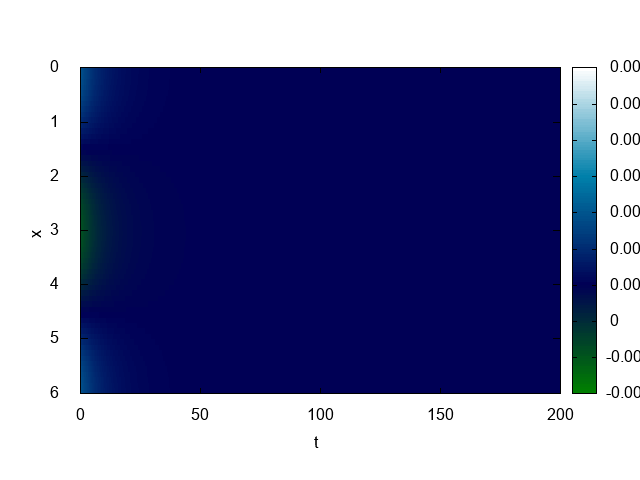
\includegraphics[scale=0.45]{plot-u-6-3.png}
                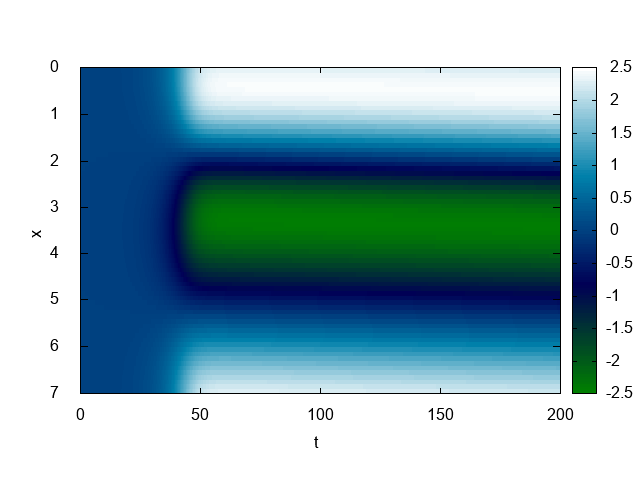
\includegraphics[scale=0.45]{plot-u-7-3.png}
                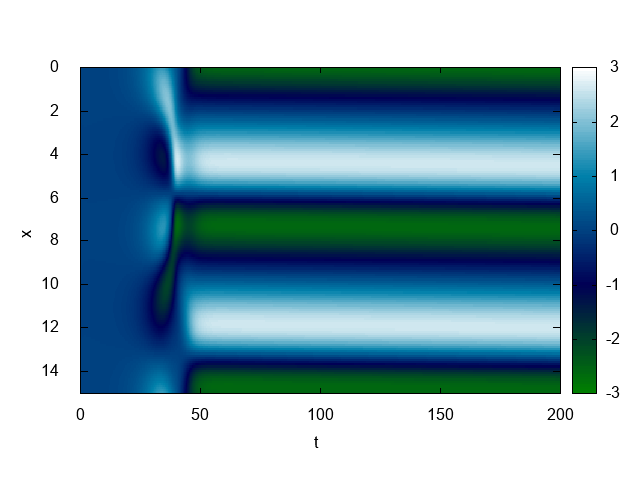
\includegraphics[scale=0.45]{plot-u-15-9.png}\\
                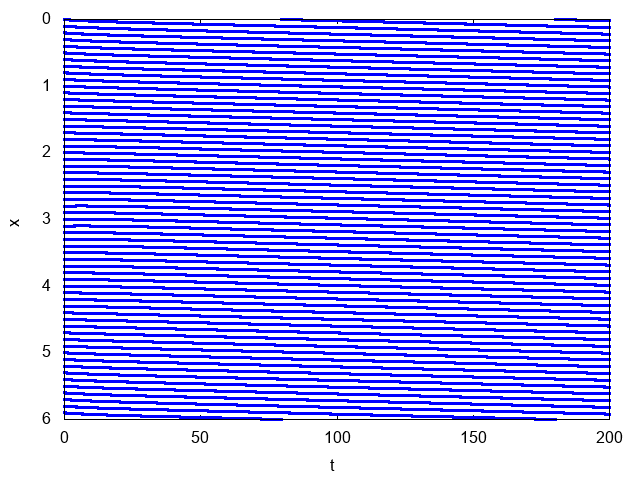
\includegraphics[scale=0.45]{plot-x-6-3.png}
                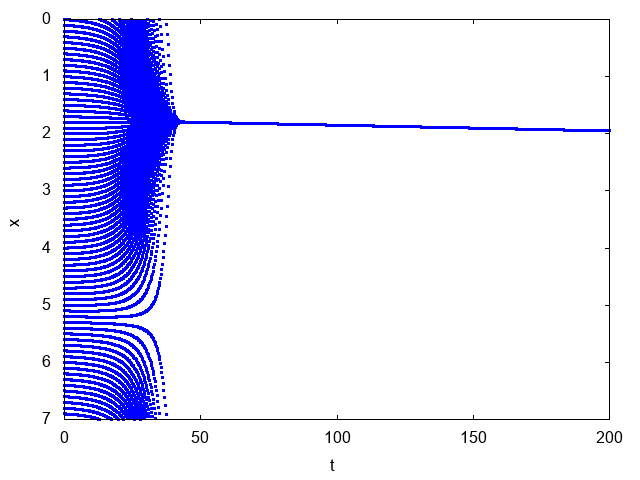
\includegraphics[scale=0.45]{plot-x-7-3.png}
                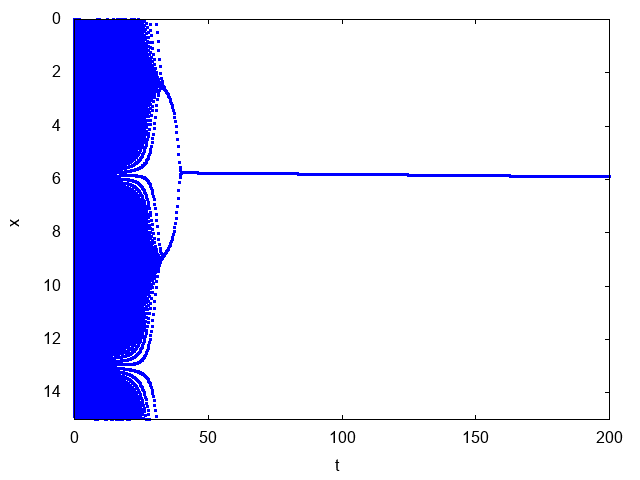
\includegraphics[scale=0.45]{plot-x-15-9.png}
                \caption{The first three plots are 3D plots and the other ones are the paths of particles. We used here $ L = 6, 7, 15 $ and $ N = 3, 3, 9$, from top to down, the values of $ L $ are growing. We get stable wavetrains. The blue dots(particles) following the wave train in the positive $ \nx $ direction. }
                \label{pic:stable}
        \end{center}
\end{figure}

\newpage

\subsection{Turbulent waves}\label{sec:turbulent}
We used the same parameter range of the last section \ref{sec:stable}, but
\begin{align*}
         L = 20, 27, 40, 64 \quad N = 9, 12, 19, 30
\end{align*} 
The result is shown in the figure \ref{pic:turbulent}.
At the beginning of $ L = 20 $, we see some deformations of the waves, but they are still stable for a period.
The width of the waves are getting smaller with increasing of $ L $. 
When we increase the parameter to $ L = 27  $, then we get more deformations and the flowing becomes turbulent. 
As we saw before, the particles are following the wave trains at the midpoint with a moving in the $ \nx $ direction. 
The range of values of velocity are $ \nnu \in [-4,4] $ and is constant in the increment of parameter $ L $. 

\begin{figure}[htp!]
        \begin{center}
        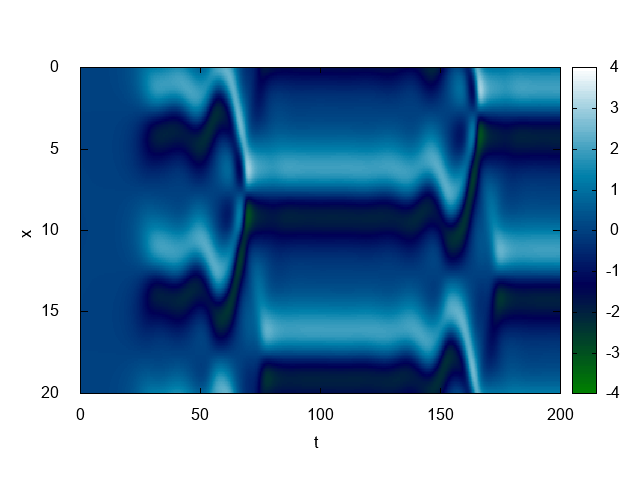
\includegraphics[scale=0.45]{plot-u-20-9.png}
        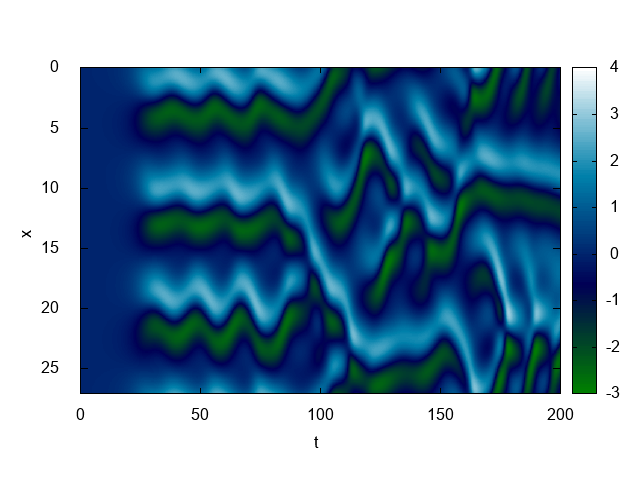
\includegraphics[scale=0.45]{plot-u-27-12.png}
        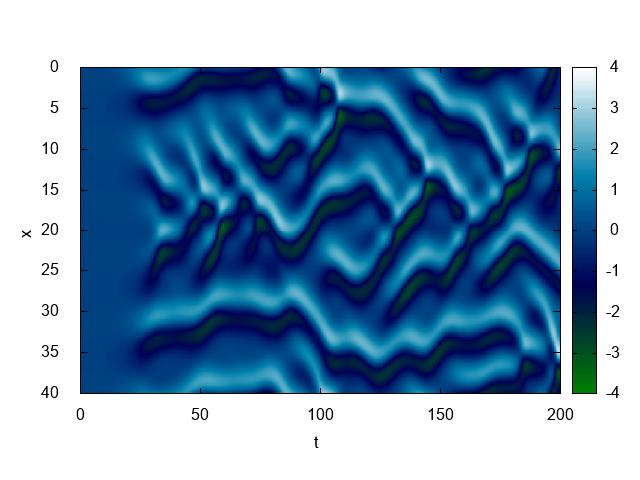
\includegraphics[scale=0.45]{plot-u-40-19.png}
        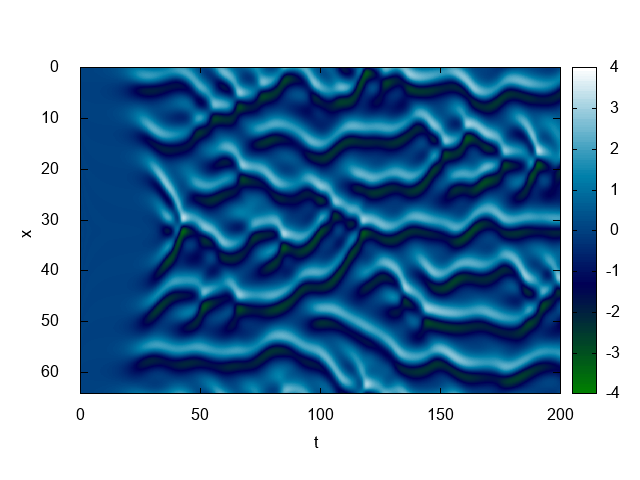
\includegraphics[scale=0.45]{plot-u-64-30.png}\\
        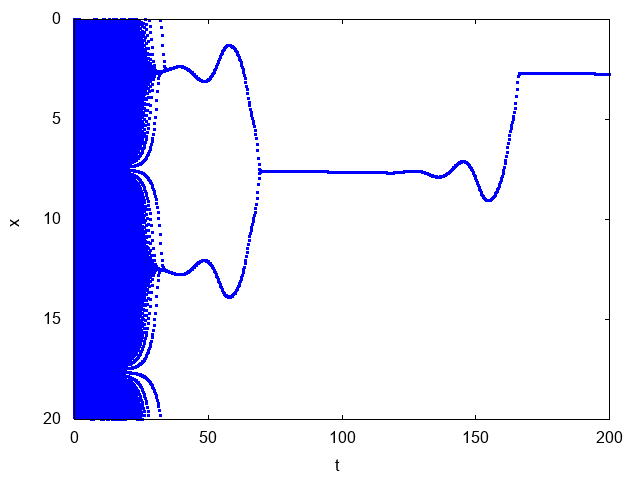
\includegraphics[scale=0.45]{plot-x-20-9.png}
        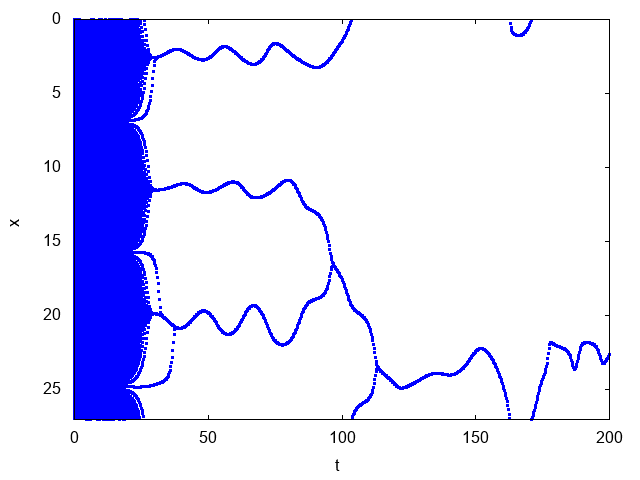
\includegraphics[scale=0.45]{plot-x-27-12.png}
        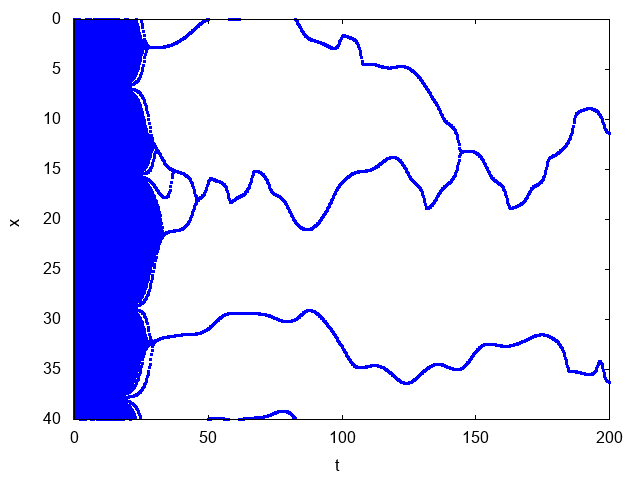
\includegraphics[scale=0.45]{plot-x-40-19.png}
        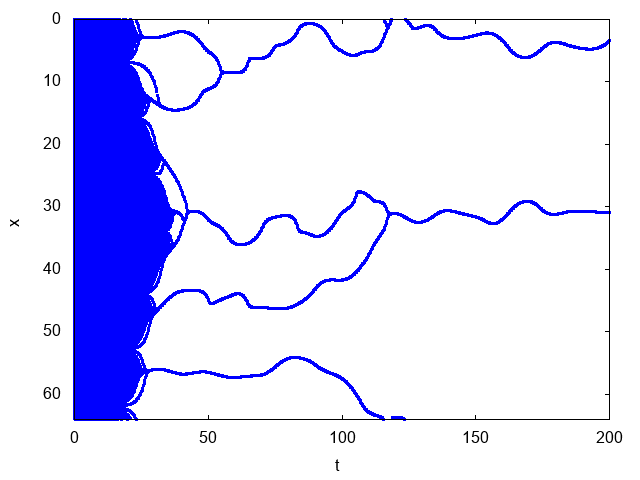
\includegraphics[scale=0.45]{plot-x-64-30.png}
        \caption{As before, the first three plots are 3D plots and the other ones are the paths of particles. We used here $ L = 20, 27, 40, 64 $ and $ N = 9, 12, 19, 30$, from top to down, the values of $ L $ are growing. We increased the parameter $ L $ and get here a turbulent flow. }
        \label{pic:turbulent}
        \end{center}
\end{figure}

\newpage

\subsection{Dependency of number of coefficients }\label{sec:coeff}
We want to investigate the dependency of number of coefficients. 
For that task we change the parameter $ N $ and the parameter $ L $ is constant. 
We used the following list of parameter
\begin{align*}
\Delta \nt = 10^{-3},\; \nt_{\mathrm{end}} = 350,\; \Delta \nx = 0.1,\; \nC_{\nn}(0) =  0.001,\; L = 27,\; N = 6, 7, 10, 19
\end{align*}
In case of $ N = 6 $, we have high amplitudes of $ \nnu $ and a fast changing of the turbulent flow.
In case of $ N > 6 $, we have a turbulent flow, but at specific times, there are stable wave fronts with small oscillations.
Below $ N < 6 $, there exists no stable simulations, after a short time, the amplitude of $ \nnu $ goes to infinity. 
There are more unstable then stable ones, because of the formula \eqref{eq:n_gr_max} for the number of growing modes
\begin{align*}
        \nn_{\mathrm{grow}} = \frac{L}{2\pi} \approx 4.2972
\end{align*}
Hence, we need more stable modes above this value.
\begin{figure}[htp!]
        %\begin{center}
                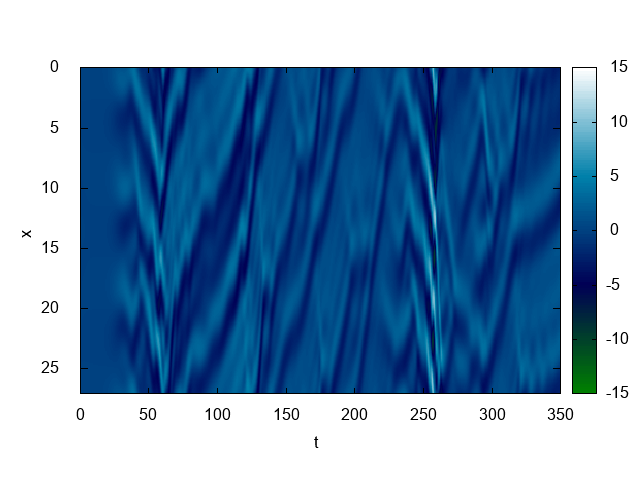
\includegraphics[scale=0.5]{plot-u-27-6.png}
                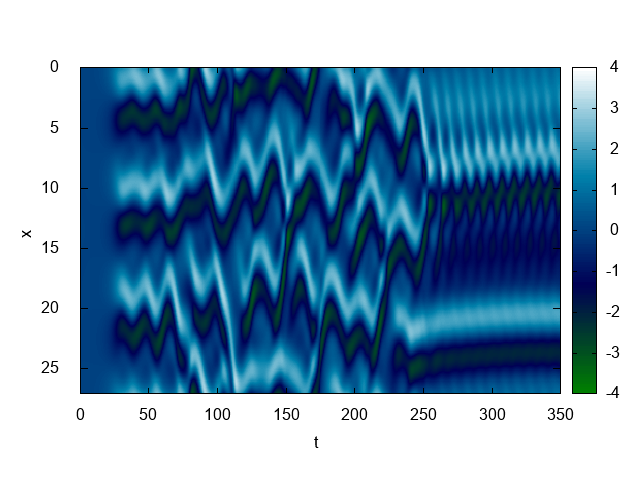
\includegraphics[scale=0.5]{plot-u-27-7.png}
                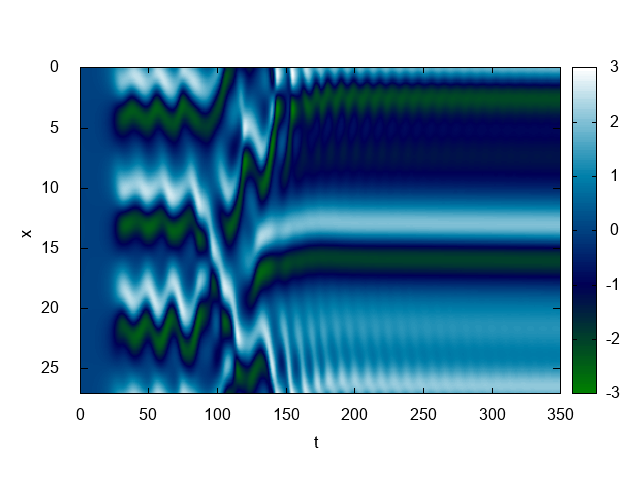
\includegraphics[scale=0.5]{plot-u-27-10.png}
                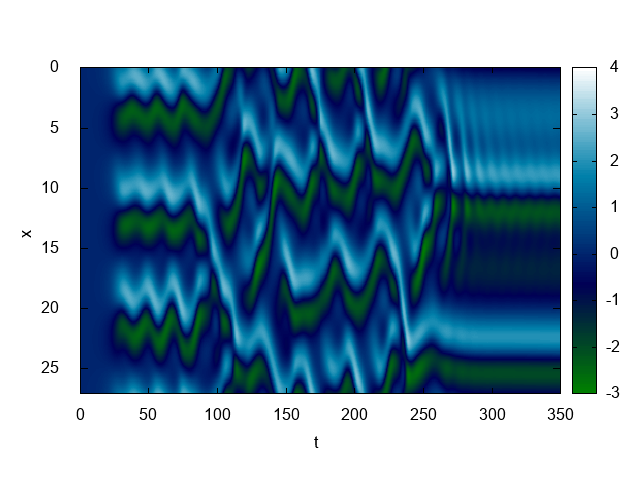
\includegraphics[scale=0.5]{plot-u-27-19.png}
                \caption{We used here $ L = 27 $ and $ N = 6, 7, 10, 19$, from top to down, the values of $ N $ are growing. We increased the parameter $ N $ and get here a turbulent flow, that sometimes stabilizes at a specific time with small oscillations.}
                \label{pic:coeff}
        %\end{center}
\end{figure}

\newpage

\section{Conclusion}
We found, that the flow is depended on the parameters $ L $ and $ N $. 
$ L $ is the width of the simulation and $ N $ the half number of modes.
 In case of $ L < 20 $, we have stable waves with no turbulence. 
 In case of $ L \geq 20 $, the flowing becomes unstable and it produces turbulence. 
The parameter $ N $ changes the number of modes.
In the theory part we found, that we get stable and unstable modes.
 In case of $ N \leq \nn_{\mathrm{grow}} $, the simulation becomes unstable, hence we have not enough stable modes to compensate the unstable modes. 
 In case of $ N > \nn_{\mathrm{grow}} $, the simulation becomes stable.
 When we distribute on that flow some particles, we can tracking them to their final destination. 
 They follow the wave fronts in positive directions and after some time all particles are collected at a wave. 

\newpage

\section{Program}
The code is written in the programming language Julia (\url{https://julialang.org/}).
You can see the code below this chapter, where you can find some annotations for clarification. 
The program has some parameter.
\begin{verbatim}
   julia falling-liquid-films.jl p1 p2 p3 p4 p5 p6 p7 p8
   
   p1 - L, lenght of the cell 
   p2 - N, half number of modes 
   p3 - delta_t, time step 
   p4 - limit_t, end time of the simulation
   p5 - delta_x, x direction steps
   p6 - schalter, choice between: live plot value=1 and save computed data value=0  
   p7 - C_n(0), start value for all avaible modes
   p8 - out_time, time step for the calculation of velocity field u
\end{verbatim}
An example execution command is
\begin{verbatim}
        julia falling-liquid-films.jl 20 18 1e-3 200 1e-1 0 0.01 0.5
\end{verbatim}
In the live plot mode you have to use the command
\begin{verbatim}
        julia falling-liquid-films.jl 20 18 1e-3 200 1e-1 1 0.01 0.5 | gnuplot 
\end{verbatim}
\nwenddocs{}\nwbegindocs{2}\nwdocspar
\nwenddocs{}\nwbegincode{3}\sublabel{NW3ZfrOy-1i61f6-1}\nwmargintag{{\nwtagstyle{}\subpageref{NW3ZfrOy-1i61f6-1}}}\moddef{falling-liquid-films.jl~{\nwtagstyle{}\subpageref{NW3ZfrOy-1i61f6-1}}}\endmoddef\nwstartdeflinemarkup\nwenddeflinemarkup
# Falling liquid films: Kuramoto-Sivashinsky equation program

\LA{}Output~{\nwtagstyle{}\subpageref{NW3ZfrOy-2r7wy0-1}}\RA{}
\LA{}Init~{\nwtagstyle{}\subpageref{NW3ZfrOy-13rLI-1}}\RA{}
\LA{}XPoints~{\nwtagstyle{}\subpageref{NW3ZfrOy-36nnlL-1}}\RA{}
\LA{}FunctionU~{\nwtagstyle{}\subpageref{NW3ZfrOy-RhCa0-1}}\RA{}
\LA{}CompCoeff~{\nwtagstyle{}\subpageref{NW3ZfrOy-49A5Z-1}}\RA{}
\LA{}CompAdvect~{\nwtagstyle{}\subpageref{NW3ZfrOy-b0Ok4-1}}\RA{}
\LA{}CompSingAdvect~{\nwtagstyle{}\subpageref{NW3ZfrOy-2yNLzt-1}}\RA{}
\LA{}CompVelo~{\nwtagstyle{}\subpageref{NW3ZfrOy-2ldCCn-1}}\RA{}
\LA{}NumCalc~{\nwtagstyle{}\subpageref{NW3ZfrOy-3QhXhc-1}}\RA{}

# Execution of algorithm to simulate the falling liquid films.

Init()

CompCoeff()

NumCalc()

\nwnotused{falling-liquid-films.jl}\nwendcode{}\nwbegindocs{4}\nwdocspar
The output function for gnuplot program

\nwenddocs{}\nwbegincode{5}\sublabel{NW3ZfrOy-2r7wy0-1}\nwmargintag{{\nwtagstyle{}\subpageref{NW3ZfrOy-2r7wy0-1}}}\moddef{Output~{\nwtagstyle{}\subpageref{NW3ZfrOy-2r7wy0-1}}}\endmoddef\nwstartdeflinemarkup\nwusesondefline{\\{NW3ZfrOy-1i61f6-1}}\nwenddeflinemarkup

function output(channel, data1, data2, data3 )
   if channel == 1
      write(single_particle_file,"$data1 $data2 $data3 \\n")
   elseif channel == 2
      write(xtrajectory_file,"$data1 $data2 $data3 \\n")
   elseif channel == 3
      write(data_file,"$data1 $data2 $data3 \\n")
   elseif (channel == 4 && schalter == 1 )
      println("$data1 $data2 $data3")
   end
end

\nwused{\\{NW3ZfrOy-1i61f6-1}}\nwendcode{}\nwbegindocs{6}\nwdocspar
Initialization of the starting parameter.
The boundary conditions for $\nC_{\nn} (0)$ are arbitrary.

\nwenddocs{}\nwbegincode{7}\sublabel{NW3ZfrOy-13rLI-1}\nwmargintag{{\nwtagstyle{}\subpageref{NW3ZfrOy-13rLI-1}}}\moddef{Init~{\nwtagstyle{}\subpageref{NW3ZfrOy-13rLI-1}}}\endmoddef\nwstartdeflinemarkup\nwusesondefline{\\{NW3ZfrOy-1i61f6-1}}\nwenddeflinemarkup
function Init()

   global L = parse(Int, ARGS[1] )# length of the x direction
   global N = parse(Int, ARGS[2] )# number of modes
   global M = 2*N+1
   global delta_t = parse(Float64, ARGS[3] )# time step
   global limit_t = parse(Float64, ARGS[4] )# time of simulation
   global delta_x = parse(Float64, ARGS[5] )# x step
   global x = Float64[0:delta_x:L;] # grid for x plotting
   global xsize = length(x )
   global C = complex(zeros(Float64, M ) ) # complex coefficients C_n
   fill!( C, parse(Float64, ARGS[7] )) # start points of C_n(0) at t = 0
   global F = complex(zeros(Float64, M ) )# function for the nonlinear terms
   global X = zeros(Float64, xsize ) # particles in the flow
   global Y = zeros(Float64, xsize ) # particles in the flow
   global out_time = parse(Float64, ARGS[8] )
   global schalter = parse(Int, ARGS[6] ) # switch for live plotting of u,x
   global lineend = 1
   
   ### data files for the output and input
   if schalter == 0
      global data_file = open("data-$L-$N-$delta_t-$limit_t-$delta_x-$(parse(Float64, ARGS[7] ) )-$out_time.txt","w") # file for x,t,u plotting
      global xtrajectory_file = open("xtrajectory-$L-$N-$delta_t-$limit_t-$delta_x-$(parse(Float64, ARGS[7] ) )-$out_time.txt","w") # file for x trajectory plotting of x,t
      global single_particle_file = open("single_particle-$L-$N-$delta_t-$limit_t-$delta_x-$(parse(Float64, ARGS[7] ) )-$out_time.txt","w")
   else
      global data_file = open("data.txt","w") # file for x,t,u plotting
      global xtrajectory_file = open("xtrajectory.txt","w") # file for x trajectory plotting of x,t
      global single_particle_file = open("single_particle.txt","w")
   end
   global xstart_file = open("xstart.txt")# file for positions of particles 
    
   output(1, "#$(parse(Int,ARGS[1]))-$(parse(Int,ARGS[2]))-\\\\
#$(parse(Float64,ARGS[3]))-$(parse(Float64,ARGS[4]))-\\\\
#$(parse(Float64,ARGS[5]))-$(parse(Int,ARGS[6]))-\\\\
#$(parse(Float64,ARGS[7])))", " ", " ")
   output(2, "#$(parse(Int,ARGS[1]))-$(parse(Int,ARGS[2]))-\\\\
#$(parse(Float64,ARGS[3]))-$(parse(Float64,ARGS[4]))-\\\\
#$(parse(Float64,ARGS[5]))-$(parse(Int,ARGS[6]))-\\\\
#$(parse(Float64,ARGS[7])))", " ", " ")
   output(3, "#$(parse(Int,ARGS[1]))-$(parse(Int,ARGS[2]))-\\\\
#$(parse(Float64,ARGS[3]))-$(parse(Float64,ARGS[4]))-\\\\
#$(parse(Float64,ARGS[5]))-$(parse(Int,ARGS[6]))-\\\\
#$(parse(Float64,ARGS[7])))", " ", " ") 
   output(4, "set yrange [-6:6]", " ", " " )
   
   # setup a number of particles 
   XPoints()
end

\nwused{\\{NW3ZfrOy-1i61f6-1}}\nwendcode{}\nwbegindocs{8}\nwdocspar
The setup of a number of particles, that follow the stream. 

\nwenddocs{}\nwbegincode{9}\sublabel{NW3ZfrOy-36nnlL-1}\nwmargintag{{\nwtagstyle{}\subpageref{NW3ZfrOy-36nnlL-1}}}\moddef{XPoints~{\nwtagstyle{}\subpageref{NW3ZfrOy-36nnlL-1}}}\endmoddef\nwstartdeflinemarkup\nwusesondefline{\\{NW3ZfrOy-1i61f6-1}}\nwenddeflinemarkup
function XPoints()
   # starting points of the grid
   for j in 0:xsize-1
      Y[j+1]=x[j+1]
   end
   # starting points for specifig number of particles, definied in the xstart file
   global lineend = 1
   while !eof(xstart_file)
     X[lineend] = parse(Float64, readline(xstart_file ) )
     #println("$lineend $X[lineend]")
     lineend += 1
   end
end

\nwused{\\{NW3ZfrOy-1i61f6-1}}\nwendcode{}\nwbegindocs{10}\nwdocspar

Calculation of the velocity $\nnu (\nt, \nx)$ 
\begin{align*}
        \nnu (\nt, \nx) &= \sum_{\nn=-\infty}^{\infty} \nC_{\nn}(\nt) \nexp \left( i\nn \frac{2\pi}{L} \nx \right) 
        %\nC_{\nn} (\nt) &= \frac{1}{L} \int_{0}^{L} \dif \nx \; \nnu (\nt, \nx) \nexp \left( -i\nn \frac{2\pi}{L} \nx \right) \quad \nC_{-\nn} = \nC_{\nn}^{*} 
\end{align*}

We used here a Galerkin approximation in the number of modes of $\nC_{\nn} (\nt)$

\nwenddocs{}\nwbegincode{11}\sublabel{NW3ZfrOy-RhCa0-1}\nwmargintag{{\nwtagstyle{}\subpageref{NW3ZfrOy-RhCa0-1}}}\moddef{FunctionU~{\nwtagstyle{}\subpageref{NW3ZfrOy-RhCa0-1}}}\endmoddef\nwstartdeflinemarkup\nwusesondefline{\\{NW3ZfrOy-1i61f6-1}}\nwenddeflinemarkup
function FunctionU(x)
   u = complex(Float64(0 ) )
   for ne in 1:M
         if (ne > N+1)
            u = u + conj(C[2*N+2-ne])*exp(im*(ne-1-N )*2*pi*x/L )
         elseif (ne <= N+1)
            u = u + (C[ne])*exp(im*(ne-1-N )*2*pi*x/L )
         end
      end
   return u
end

\nwused{\\{NW3ZfrOy-1i61f6-1}}\nwendcode{}\nwbegindocs{12}\nwdocspar
We want to compute the $\nC_{\nn} (\nt)  $ Coefficients for the Fouriertransformation. We used the complex coefficients. Usually, the index of coefficients goes from negative to positive values of $ \nn $, then we shift the index from $ \nn \in [-N,N] $ to $ \nn \in [1,2N+1] $.

\nwenddocs{}\nwbegincode{13}\sublabel{NW3ZfrOy-49A5Z-1}\nwmargintag{{\nwtagstyle{}\subpageref{NW3ZfrOy-49A5Z-1}}}\moddef{CompCoeff~{\nwtagstyle{}\subpageref{NW3ZfrOy-49A5Z-1}}}\endmoddef\nwstartdeflinemarkup\nwusesondefline{\\{NW3ZfrOy-1i61f6-1}}\nwenddeflinemarkup
function CompCoeff()
   for ne in 1:N
      C[N+1-ne]=conj(C[N+1+ne] )
   end
   for ne in 2+N:M
      F[ne] = 0
      for l in ne-N:M
         F[ne] = F[ne] + C[l] * C[ne-l+N+1]
      end
      F[ne]=-F[ne]*im*(ne-N-1)*pi/L
   end
end

\nwused{\\{NW3ZfrOy-1i61f6-1}}\nwendcode{}\nwbegindocs{14}\nwdocspar

Calculation of the path of the particles. They follow the velocity law 

\begin{align*}
        \frac{\dif \nX}{\dif \nt} = \nnu (\nX, \nt)
\end{align*}

We used the simple Euler method to compute the path of the particles. This method is sufficient, because we only have calculated two points in one time step with the chosen method (ETD2RK). 

\begin{align*}
        \nX _{\nm+1} = \nX _{\nm} + \Delta \nt \nnu (\nX_{\nm}, \nt_{\nm})
\end{align*}

\nwenddocs{}\nwbegincode{15}\sublabel{NW3ZfrOy-b0Ok4-1}\nwmargintag{{\nwtagstyle{}\subpageref{NW3ZfrOy-b0Ok4-1}}}\moddef{CompAdvect~{\nwtagstyle{}\subpageref{NW3ZfrOy-b0Ok4-1}}}\endmoddef\nwstartdeflinemarkup\nwusesondefline{\\{NW3ZfrOy-1i61f6-1}}\nwenddeflinemarkup
function CompAdvect(t,j)
   Y[j+1]=Y[j+1] + out_time*real(FunctionU(Y[j+1] ) )
   if Y[j+1]>L
      Y[j+1]=Y[j+1]-L
   elseif Y[j+1]<0
      Y[j+1]=Y[j+1]+L
   end
   output(2, t, Y[j+1], " " )
end

\nwused{\\{NW3ZfrOy-1i61f6-1}}\nwendcode{}\nwbegindocs{16}\nwdocspar
Computation of the velocity $ \nnu (\nt, \nx)$

\nwenddocs{}\nwbegincode{17}\sublabel{NW3ZfrOy-2ldCCn-1}\nwmargintag{{\nwtagstyle{}\subpageref{NW3ZfrOy-2ldCCn-1}}}\moddef{CompVelo~{\nwtagstyle{}\subpageref{NW3ZfrOy-2ldCCn-1}}}\endmoddef\nwstartdeflinemarkup\nwusesondefline{\\{NW3ZfrOy-1i61f6-1}}\nwenddeflinemarkup
function CompVelo(t)
   output(4, "plot '-' using 2:3 w l", " ", " " )
   for j in 0:xsize-1 #x direction steps
      w::Float64 = real(FunctionU(x[j+1] ) )
      output(3, t, j*delta_x, w )
      output(4, t, j*delta_x, w )
      
      CompAdvect(t,j)
   end
   output(2, " ", " ", " " )
   output(3, " ", " ", " " )
   output(4, "eol: 0", " ", " " )
end

\nwused{\\{NW3ZfrOy-1i61f6-1}}\nwendcode{}\nwbegindocs{18}\nwdocspar
The function computes the path of particles, that was given by a list of starting positions in the file \texttt{xstart.txt}.

\nwenddocs{}\nwbegincode{19}\sublabel{NW3ZfrOy-2yNLzt-1}\nwmargintag{{\nwtagstyle{}\subpageref{NW3ZfrOy-2yNLzt-1}}}\moddef{CompSingAdvect~{\nwtagstyle{}\subpageref{NW3ZfrOy-2yNLzt-1}}}\endmoddef\nwstartdeflinemarkup\nwusesondefline{\\{NW3ZfrOy-1i61f6-1}}\nwenddeflinemarkup
function CompSingAdvect(t)
   for j in 1:lineend
      X[j]=X[j] + out_time*real(FunctionU(X[j] ) )
      if X[j]>L
         X[j]=X[j]-L
      elseif X[j]<0
         X[j]=X[j]+L
      end
      output(1, t, X[j], " " )
   end
   output(1, " ", " ", " " )
end

\nwused{\\{NW3ZfrOy-1i61f6-1}}\nwendcode{}\nwbegindocs{20}\nwdocspar
Numerical solution of the system of ordinary differential equations for $ \nC_{\nn} (\nt) $

\nwenddocs{}\nwbegincode{21}\sublabel{NW3ZfrOy-3QhXhc-1}\nwmargintag{{\nwtagstyle{}\subpageref{NW3ZfrOy-3QhXhc-1}}}\moddef{NumCalc~{\nwtagstyle{}\subpageref{NW3ZfrOy-3QhXhc-1}}}\endmoddef\nwstartdeflinemarkup\nwusesondefline{\\{NW3ZfrOy-1i61f6-1}}\nwenddeflinemarkup
function NumCalc()
   Fe = complex(zeros(Float64, M ) )
   for t in 0:delta_t:limit_t
      Ce = complex(zeros(Float64, M ) )
      for ne in N+2:M
         a = Float64(((ne-N-1)*2*pi/L )^2-((ne-N-1)*2*pi/L )^4 )
         Fe[ne]=F[ne]
         Ce[ne] = C[ne]*exp(a*delta_t) + F[ne]*(exp(a*delta_t )-1 )/a
      end
      
      CompCoeff()
      
      for ne in N+2:M
         a = Float64(((ne-N-1 )*2*pi/L )^2-((ne-N-1 )*2*pi/L )^4 )
         C[ne] = Ce[ne] + (F[ne]-Fe[ne] )*(exp(a*delta_t ) -1 - a*delta_t )/(a^2*delta_t )
      end
      if (trunc(mod(t*1e4, out_time*1e4)) == 0 )
         CompVelo(t)
         CompSingAdvect(t)
      end
   end
end

\nwused{\\{NW3ZfrOy-1i61f6-1}}\nwendcode{}\nwbegindocs{22}\nwdocspar

\begin{comment}

\nwenddocs{}\nwbegindocs{23}\nwdocspar
June 2019

1| 2| 3| 4| *5| 1-2s1 *6| 1-2s1 7| 8| *9| 1-3s1 *10| 1-7s1 *11| 1-3s1 12| *13| 1-3s1 *14| 1-4s1 15| 16| *17| 1-4s1 18| *19| 1-2s1 *20| 1-2s1 *21| 1s1-2 22| *23| 1s1 *24| 1s0-3 *25| 1s1-2 *26| 1s1 27| 28| 29| 30| 31|

July 2019

1| *2| 3| *4| *5| 6| *7| *8| *9| *10| 11| 12| 13| 14| 15| 16| 17| *18| *19| 20| 21| 22| 23| 24| 25| 26| 27| 28| 29| 30| 31|
@language python
from subprocess import call
# Methode zum Erzeugen des Programm Quellcodes
print('--------------------------<')
print('Running program')
g.execute_shell_commands("notangle -Rliquid-rocket.sh falling-liquid-films.nw > liquid-rocket.sh")
g.execute_shell_commands("notangle -R3dplot-t,x,u.plt falling-liquid-films.nw > 3dplot-t,x,u.plt")
g.execute_shell_commands("notangle -Rx-trajectory.plt falling-liquid-films.nw > x-trajectory.plt")
g.execute_shell_commands("./liquid-rocket.sh &")
##### Meta
'''
Programmiersprache: julia
Methoden:
    - 
'''

##### History
'''
Program hits:
July 2019

1| *2| 3| *4| *5| 6| *7| *8| *9| *10| 11| 12| 13| 14| 15| 16| 17| 18| 19| 20| 21| *22| 23| 24| 25| 26| 27| 28| 29| 30| 31|
   
June 2019

1| 2| 3| 4| 5| 6| 7| 8| 9| 10| 11| 12| 13| 14| 15| *16| *17| *18| *19| *20| *21| 22| *23| *24| *25| *26| *27| *28| *29| 30| 31|

memorable doings:
22.7.2019
   - completed all sections and references
19.7.2019
   - completed section simulation
9.7.2019
   - some corrections in protocol
   - plotting for the protocol 
8.7.2019
   - almost complete theory part
7.7.2019
   - rewrite of the program in computation of the values of the velocity
   - new function for a specific number of single particles
5.7.2019
   - complete turbolent program, now it works correctly
   - the x trajectories working correctly
26.5.2019
   - corrected program and it runs correctly (I think so)
   - outline of the whole work
25.6.2019
   - reduced coefficients to N
   - calculation of X and u works, but it is not the right result
20.6.2019
   - first functional version of the program
19.6.2019
   - right calculation of the coefficients (I think so)
      - program first algorithm
      - writed
18.6.2019
   - initiation of the project folder 
    
'''

print('-------------------------->')

\nwenddocs{}\nwbegindocs{24}\nwdocspar
@language python
from subprocess import call
# Methode zum Erzeugen des Programm Quellcodes
print('--------------------------<')
print('Running program')
g.execute_shell_commands("notangle -Rliquid-rocket.sh falling-liquid-films.nw > liquid-rocket.sh")
g.execute_shell_commands("notangle -R3dplot-t,x,u.plt falling-liquid-films.nw > 3dplot-t,x,u.plt")
g.execute_shell_commands("notangle -Rx-trajectory.plt falling-liquid-films.nw > x-trajectory.plt")
g.execute_shell_commands("./liquid-rocket.sh &")
##### Meta
'''
Programmiersprache: julia
Methoden:
    - 
'''

##### History
'''
Program hits:
July 2019

1| *2| 3| *4| *5| 6| *7| *8| *9| *10| 11| 12| 13| 14| 15| 16| 17| 18| 19| 20| 21| *22| 23| 24| 25| 26| 27| 28| 29| 30| 31|
   
June 2019

1| 2| 3| 4| 5| 6| 7| 8| 9| 10| 11| 12| 13| 14| 15| *16| *17| *18| *19| *20| *21| 22| *23| *24| *25| *26| *27| *28| *29| 30| 31|

memorable doings:
22.7.2019
   - completed all sections and references
19.7.2019
   - completed section simulation
9.7.2019
   - some corrections in protocol
   - plotting for the protocol 
8.7.2019
   - almost complete theory part
7.7.2019
   - rewrite of the program in computation of the values of the velocity
   - new function for a specific number of single particles
5.7.2019
   - complete turbolent program, now it works correctly
   - the x trajectories working correctly
26.5.2019
   - corrected program and it runs correctly (I think so)
   - outline of the whole work
25.6.2019
   - reduced coefficients to N
   - calculation of X and u works, but it is not the right result
20.6.2019
   - first functional version of the program
19.6.2019
   - right calculation of the coefficients (I think so)
      - program first algorithm
      - writed
18.6.2019
   - initiation of the project folder 
    
'''

print('-------------------------->')

\nwenddocs{}\nwbegindocs{25}\nwdocspar
@language shell
\nwenddocs{}\nwbegincode{26}\sublabel{NW3ZfrOy-2bsYZX-1}\nwmargintag{{\nwtagstyle{}\subpageref{NW3ZfrOy-2bsYZX-1}}}\moddef{liquid-rocket.sh~{\nwtagstyle{}\subpageref{NW3ZfrOy-2bsYZX-1}}}\endmoddef\nwstartdeflinemarkup\nwenddeflinemarkup
echo '----------------Start Program----------------'

#### comiplation and producing of the output

notangle -Rfalling-liquid-films.jl falling-liquid-films.nw > falling-liquid-films.jl
notangle -R3dplot-t,x,u.plt falling-liquid-films.nw > 3dplot-t,x,u.plt
notangle -Rx-trajectory.plt falling-liquid-films.nw > x-trajectory.plt
notangle -Rxstart.txt falling-liquid-films.nw > xstart.txt

#### parameter overview
#                              L     N     delta_t     limit_t     delta_x     schalter     C_n(0)     output time
#julia falling-liquid-films.jl p1(L) p2(N) p3(delta_t) p4(limit_t) p5(delta_x) p6(schalter) p7(C_n(0)) p8(output time)

#### programming tasks
: '
0:
+  checking the right solution
1:
+  use for N the triple number of unstable modes
+  3D plot
+  show for L >= 20 solutions are turbulent
|  dependancy of the number of modes N

2:
+  particle plot of the final stage of the evolution
+  a good plot of particles path
+  a free choosable start point for a particle

'


#### computation

## compilation of interesting plots

# nice patterns and turbulently flow
#time julia falling-liquid-films.jl 64 40 1e-3 200 1e-1 1 0.001 0.25 | gnuplot -p

#stable wave
#time julia falling-liquid-films.jl 10 8 1e-3 140 1e-1 1 0.01 0.3 | gnuplot -p

#also nice plots
#time julia falling-liquid-films.jl 25 12 1e-3 280 1e-1 1 0.005 0.25 | gnuplot -p

# nice turbulents at L = 50 and particle trajectories
#time julia falling-liquid-films.jl 50 30 1e-3 140 1e-1 1 0.01 0.3 | gnuplot -p

# the beginnings of turbulents
#time julia falling-liquid-films.jl 20 10 1e-2 217.5 1e-1 1 0.005 0.25 | gnuplot -p

#also interesting turbulents
#time julia falling-liquid-films.jl 25 12 1e-3 280 1e-1 1 0.005 0.25 | gnuplot -p

# some more 'orderd' turbulents
#time julia falling-liquid-films.jl 50 30 1e-3 240 1e-1 1 0.0001 0.3 | gnuplot -p

# also nice
#time julia falling-liquid-films.jl 30 20 1e-3 440 1e-1 1 0.5 0.2 | gnuplot -p

### tasks

## stable waves

#time julia falling-liquid-films.jl 15 5 1e-3 200 1e-1 1 0.5 0.25 | gnuplot -p

# L = 6
#time julia falling-liquid-films.jl 6 3 1e-3 200 1e-1 0 0.001 0.25 #| gnuplot -p

# L = 7
#time julia falling-liquid-films.jl 7 3 1e-3 200 1e-1 1 0.001 0.25 | gnuplot -p

# L = 10
#time julia falling-liquid-films.jl 10 6 1e-3 200 1e-1 0 0.001 0.25 #| gnuplot -p

# L = 15
#time julia falling-liquid-films.jl 15 9 1e-3 200 1e-1 0 0.001 0.25 #| gnuplot -p

## turbulent

# L = 20
# starting of turbulents
#time julia falling-liquid-films.jl 20 9 1e-3 200 1e-1 0 0.001 0.25 #| gnuplot -p

# L = 27
#time julia falling-liquid-films.jl 27 12 1e-3 200 1e-1 0 0.001 0.25 #| gnuplot -p

# L = 40
#time julia falling-liquid-films.jl 40 19 1e-3 200 1e-1 0 0.001 0.25 #| gnuplot -p

# L = 64
#time julia falling-liquid-films.jl 64 30 1e-3 200 1e-1 0 0.001 0.25 #| gnuplot -p

## dependacy on the number of modes
# 
: '
for L = 30 triple 14
n = 6 castrophe
n = 7 stable with strong piek, turbulent
n = 8 stable, turbulent
n = 9 stable, trubolent with some strong waves
n = 10 :, : 
n = 11 :, :
n = 12 :, :
n = 13 :, :
n = 

at 13 everytime the same picture

for L = 27 triple 13
n = 5 catastrophe
n = 6 very turbulent and almost unstable
n = 7 more stable, also turbulent, by C(0) = 0.001 then goes to steady state
n = 8 more stable, :
n = 9 more stable
n = 10 same
n = 11 other picture turbulent 
n = 12 same
n = 13 same
n = 14 other picture turbulent
n = 15 same it 
n = 16 very turbulent
n = 17 same
n = 18 same
n = 19 same  by C(0) = 0.001 then goes to steady state
n = 20 very turbulent
n = 21 same
n = 22 same

'
#time julia falling-liquid-films.jl 27 12 1e-3 350 1e-1 1 0.001 0.75 | gnuplot -p

###testing

time julia falling-liquid-films.jl 27 13 1e-3 350 1e-1 1 0.001 0.75 | gnuplot -p

#### Plot of data

echo '----------------Gnuplot Start----------------'
#gnuplot live-plot.txt -p &

### 3D plot for t,x,u values
gnuplot 3dplot-t,x,u.plt -p

### x trajectory plot t,x
gnuplot x-trajectory.plt -p

echo '----------------End ----------------'

\nwnotused{liquid-rocket.sh}\nwendcode{}\nwbegindocs{27}\nwdocspar
Gnuplot file for plotting the 3D plot for t,x,u.

\nwenddocs{}\nwbegincode{28}\sublabel{NW3ZfrOy-gK3Zg-1}\nwmargintag{{\nwtagstyle{}\subpageref{NW3ZfrOy-gK3Zg-1}}}\moddef{3dplot-t,x,u.plt~{\nwtagstyle{}\subpageref{NW3ZfrOy-gK3Zg-1}}}\endmoddef\nwstartdeflinemarkup\nwenddeflinemarkup
reset
set pm3d map
unset grid
set xlabel "t "
set ylabel "x "
set zlabel "u "
#set yrange [6:0] reverse
set yrange [*:*] reverse
set palette rgb 23,28,3; #set title "ocean (green-blue-white)\\ntry also other permutations";
#set view 28, 6
# every :::(first block)::(last block)
splot 'data.txt' using 1:2:3 with pm3d notitle
#set term png
# #'plot-u-L-n.pdf'
#set output 'plot-u-6-3.png'
#splot 'data-6-3-0.001-200.0-0.1-0.001-0.25.txt' using ($1):($2):($3) with pm3d notitle
#set term qt
#replot
\nwnotused{3dplot-t,x,u.plt}\nwendcode{}\nwbegindocs{29}\nwdocspar
Gnuplot file for plotting the x trajectory in t,x.

\nwenddocs{}\nwbegincode{30}\sublabel{NW3ZfrOy-3CPUEO-1}\nwmargintag{{\nwtagstyle{}\subpageref{NW3ZfrOy-3CPUEO-1}}}\moddef{x-trajectory.plt~{\nwtagstyle{}\subpageref{NW3ZfrOy-3CPUEO-1}}}\endmoddef\nwstartdeflinemarkup\nwenddeflinemarkup
reset
#set key outside rmargin
set key off
set xlabel "t "
set ylabel "x "
set yrange [*:*] reverse
#set yrange [6:0] reverse
# every :::(first block)::(last block)
# every ::(first line):::(last line)
# every :::1::50
plot 'xtrajectory.txt' using ($1):($2) ps 0.4 pt 5 lc rgb 'blue' #title ' '.i.'. x'
#set term png
# #'plot-x-L-n.pdf'
#set output 'plot-x-6-3.png'
#plot 'xtrajectory-6-3-0.001-200.0-0.1-0.001-0.25.txt' using ($1):($2) ps 0.3 pt 5 lc rgb 'blue' notitle
#set term qt
#replot
\nwnotused{x-trajectory.plt}\nwendcode{}\nwbegindocs{31}\nwdocspar
The starting points of the particles.

\nwenddocs{}\nwbegincode{32}\sublabel{NW3ZfrOy-3ix8kZ-1}\nwmargintag{{\nwtagstyle{}\subpageref{NW3ZfrOy-3ix8kZ-1}}}\moddef{xstart.txt~{\nwtagstyle{}\subpageref{NW3ZfrOy-3ix8kZ-1}}}\endmoddef\nwstartdeflinemarkup\nwenddeflinemarkup
1
2
3
4
\nwnotused{xstart.txt}\nwendcode{}\nwbegindocs{33}\nwdocspar
@language python
##### Programm zum Start der Versionisierung des Codes
from subprocess import call
print('--------------------------<')
print('Commiting a new version of falling-liquid-films.nw')
g.execute_shell_commands("notangle -RVersions.conf falling-liquid-films.nw > Versions.conf &")
g.execute_shell_commands("/home/christian/Programme/storeBackup/bin/storeBackup.pl -f Versions.conf &")
print('-------------------------->')

\nwenddocs{}\nwbegindocs{34}\nwdocspar
@language python
from subprocess import call
g.execute_shell_commands("konsole --workdir /home/home/christian/Gedankenspeicher/ownCloud/Comp-Physics-4/ --hold -e 'gnuplot' &")
\nwenddocs{}\nwbegincode{35}\sublabel{NW3ZfrOy-3YPuMQ-1}\nwmargintag{{\nwtagstyle{}\subpageref{NW3ZfrOy-3YPuMQ-1}}}\moddef{Versions.conf~{\nwtagstyle{}\subpageref{NW3ZfrOy-3YPuMQ-1}}}\endmoddef\nwstartdeflinemarkup\nwenddeflinemarkup

# configuration file for storeBackup.pl
# Generated by storeBackup.pl, 3.5

####################
### explanations ###
####################

# You can set a value specified with '-cf_key' (eg. logFiles) and
# continue at the next lines which have to begin with a white space:
# logFiles = /var/log/messages  /var/log/cups/access_log
#      /var/log/cups/error_log
# One ore more white spaces are interpreted as separators.
# You can use single quotes or double quotes to group strings
# together, eg. if you have a filename with a blank in its name:
# logFiles = '/var/log/my strage log'
# will result in one filename, not in three.
# If an option should have *no value*, write:
# logFiles =
# If you want the default value, comment it:
logFile = Versions-Programm.log

# You can also use environment variables, like $XXX or $\{XXX\} like in
# a shell. Single quotes will mask environment variables, while double
# quotes will not.
# You can mask $, \{, \}, ", ' with a backslash (\\), eg. \\$
# Lines beginning with a '#' or ';' are ignored (use this for comments)
#
# You can overwrite settings in the command line. You can remove
# the setting also in the command by using the --unset feature, eg.:
# '--unset doNotDelete' or '--unset --doNotDelete'

#####################
### configuration ###
#####################

# source directory (*** must be specified ***)
sourceDir=/home/home/christian/Gedankenspeicher/ownCloud/Comp-Physics-4/

# top level directory of all linked backups (*** must be specified ***)
# storeBackup must know for consistency checking where all your backups
# are. This is done to make sure that your backups are consistent if you
# used --lateLinks.
backupDir=/home/home/christian/Gedankenspeicher/ownCloud/Comp-Physics-4/

# ------------------------------------------------------------------------
# you do not need specify the options below to get a running configuration
# (but they give you more features and more control)
#


# series directory, default is 'default'
# relative path from backupDir
series=Versions

# directory for temporary file, default is /tmp
;tmpDir=

# List of other backup directories to consider for
# hard linking. Relative path from backupDir!
# Format (examples):
# backupSeries/2002.08.29_08.25.28 -> consider this backup
# or
# 0:backupSeries    -> last (youngest) backup in <backupDir>/backupSeries
# 1:backupSeries    -> first before last backup in <backupDir>/backupSeries
# n:backupSeries    -> n'th before last backup in <backupDir>/backupSeries
# 3-5:backupSeries  -> 3rd, 4th and 5th in <backupDir>/backupSeries
# all:backupSeries  -> all in <backupDir>/backupSeries
# This option is useful, if you want to explicitly hard link
# to backup series from different backups. You can specify eg. with
# 0:myBackup to the last backup of series 'myBackup'. If you specify
# backup series with otherBackupSeries, then only these backups will be
# used for hard linking.
# You can also use wildcards in series names. See documentation,
# section 'Using Wildcards for Replication' for details.
# Default value is to link to the last backup of all series stored in
# 'backupDir'.
;otherBackupSeries=

# lock file, if exist, new instances will finish if
# an old is already running, default is /tmp/storeBackup.lock
;lockFile=

# remove the lock files before deleting old backups
# default ('no') is to delete the lock file after deleting
# possible values are 'yes' and 'no'
;unlockBeforeDel=

# continue if one or more of the exceptional directories
# do not exist (no is stopping processing)
# default is 'no', can be 'yes' or 'no'
;contExceptDirsErr=

# Directories to exclude from the backup (relative path inside of the backup).
# You can use shell type wildcards.
# These directories have to be separated by space or newline.
exceptDirs=Versions

# Directories to include in the backup (relative path inside of the backup).
# You can use shell type wildcards.
# These directories have to be separated by space or newline.
;includeDirs=

# rule for excluding files / only for experienced administrators
# !!! see README file 'including / excluding files and directories'
# EXAMPLE: 
# searchRule = ( '$size > &::SIZE("3M")' and '$uid eq "hjc"' ) or
#    ( '$mtime > &::DATE("3d4h")' and not '$file =~ m#/tmp/#' )'
;exceptRule=

# For explanations, see 'exceptRule'.
;includeRule=

# write a file name .storeBackup.notSaved.bz2 with the
# names of all skipped files, default is 'no', can be 'yes' or 'no'
;writeExcludeLog=

# do not save the specified types of files, allowed: Sbcfpl
# S - file is a socket
# b - file is a block special file
# c - file is a character special file
# f - file is a plain file
# p - file is a named pipe
# l - file is a symbolic link
# Spbc can only be backed up if GNU copy is available.
;exceptTypes=

# save the specified type of files in an archive instead saving
# them directly in the file system
# use this if you want to backup those file types but your target
# file or transport (eg. sshfs or non gnu-cp) system does not support
# those types of file
#   S - file is a socket
#   b - file is a block special file
#   c - file is a character special file
#   p - file is a named pipe
#   l - file is a symbolic link
# you also have to set specialTypeArchiver when using this option
;archiveTypes=


# possible values are 'cpio', 'tar', 'none'. default is 'cpio'
# tar is not able to archive sockets
# cpio is not part of the actual posix standard any more
;specialTypeArchiver=

# Activate this option if your system's cp is a full-featured GNU
# version. In this case you will be able to also backup several
# special file types like sockets.
# Possible values are 'yes' and 'no'. Default is 'no'
cpIsGnu=yes

# make a hard link to existing, identical symlinks in old backups
# use this, if your operating system supports this (linux does)
# Possible values are 'yes' and 'no'. Default is 'no'
;linkSymlinks=

# exec job before starting the backup, checks lockFile (-L) before
# starting (e.g. can be used for rsync) stops execution if job returns
# exit status != 0
;precommand=

# exec job after finishing the backup, but before erasing of old
# backups reports if job returns exit status != 0
;postcommand=

# follow symbolic links like directories up to depth 0 -> do not
# follow links
;followLinks=

# only store the contents of file systems named by
# sourceDir and symlinked via followLinks
# possible values are 'yes' and 'no'; default is 'no'
;stayInFileSystem=

# use this only if you write your backup over a high latency line
# like a vpn over the internet
# storebackup will use more parallelization at the cost of more
# cpu power
# possible values are 'yes' and 'no'; default is 'no'
;highLatency=

# If this option is disabled, then the files in the backup will not
# neccessarily have the same permissions and owner as the originals.
# This speeds up backups on network drives a lot. Correct permissions
# are restored by storeBackupRecover.pl no matter what this option is
# set to. Default is 'no'
;ignorePerms=

# suppress (unwanted) warnings in the log files;
# to suppress warnings, the following keys can be used:
#   excDir (suppresses the warning that excluded directories
#          do not exist)
#   fileChange (suppresses the warning that a file has changed during
#              the backup)
#   crSeries (suppresses the warning that storeBackup had to create the
#            'default' series)
#   hashCollision (suppresses the warning if a possible
#                 hash collision is detected)
#   fileNameWithLineFeed (suppresses the warning if a filename
#                        contains a line feed)
#    use_DB_File (suppresses the warning that you should install
#                 perl module DB_File for better perforamnce)
#    use_MLDBM (suppresses the warning that you should install
#               perl module MLDBM if you want to use rule functions
#               MARK_DIR or MARK_DIR_REC together with option saveRAM)
#    use_IOCompressBzip2 (suppresses the warning that you should
#                         instal perl module IO::Compress::Bzip2
#                         for better performance)
#    noBackupForPeriod (suppresses warning that there are
#                       no backups for certain periods when using
#                       option keepRelative)
#  This option can be repeated multiple times on the command line.
#  Example usage in conf file:
#  suppressWarning = excDir fileChange crSeries hashCollision
#  By default no warnings are suppressed.
;suppressWarning=

# do *not* write hard links to existing files in the backup
# during the backup (yes|no)
# you have to call the program storeBackupUpdateBackup.pl
# later on your server if you set this flag to 'yes'
# you have to run storeBackupUpdateBackup.pl later - see
# description for that program
# default = no: do not write hard links
;lateLinks=

# only in combination with --lateLinks
# compression from files >= size will be done later,
# the file is (temporarily) copied into the backup
# default = no: no late compression
;lateCompress=

# repair simple inconsistencies (from lateLinks) automatically
# without requesting the action
# default = no, no automatic repair
;autorepair=

# Files with specified suffix for which storeBackup will make an md5 check
# on blocks of that file. Executed after --checkBlocksRule(n)
;checkBlocksSuffix=

# Only check files specified in --checkBlocksSuffix if there
# file size is at least this value, default is 100M
;checkBlocksMinSize=

# Block size for files specified with --checkBlocksSuffix
# default is 1M (1 megabyte)
;checkBlocksBS=

# if set, the blocks generated due to checkBlocksSuffix are compressed
# Possible values are 'check, 'yes' and 'no'. Default is 'no'
# check uses COMRESSION_CHECK (see option compressSuffix)
;checkBlocksCompr=

# Read files specified here in parallel to "normal" ones.
# This only makes sense if they are on a different disk.
# Default value is 'no'
;checkBlocksParallel=

# length of queue to store files before block checking,
# default = 1000
;queueBlock=

# Files for which storeBackup will make an md5 check depending
# on blocks of that file.
# The rules are checked from rule 1 to rule 5. The first match is used
# !!! see README file 'including / excluding files and directories'
# EXAMPLE: 
# searchRule = ( '$size > &::SIZE("3M")' and '$uid eq "hjc"' ) or
#    ( '$mtime > &::DATE("3d4h")' and not '$file =~ m#/tmp/#' )'
;checkBlocksRule0=

# Block size for option checkBlocksRule
# default is 1M (1 megabyte)
;checkBlocksBS0=

# if set to 'yes', blocks generated due to this rule will be compressed
# possible values: 'check', 'yes' or 'no', default is 'no'
# check users COMRESSION_CHECK (see option compressSuffix)
;checkBlocksCompr0=

# Filter for reading the file to treat as a blocked file
# eg.   gzip -d   if the file is compressed. Default is no read filter.
;checkBlocksRead0=

# Read files specified here in parallel to "normal" ones.
# This only makes sense if they are on a different disk.
# Default value is 'no'
;checkBlocksParallel0=

;checkBlocksRule1=
;checkBlocksBS1=
;checkBlocksCompr1=
;checkBlocksRead1=
;checkBlocksParallel1=

;checkBlocksRule2=
;checkBlocksBS2=
;checkBlocksCompr2=
;checkBlocksRead2=
;checkBlocksParallel2=

;checkBlocksRule3=
;checkBlocksBS3=
;checkBlocksCompr3=
;checkBlocksRead3=
;checkBlocksParallel3=

;checkBlocksRule4=
;checkBlocksBS4=
;checkBlocksCompr4=
;checkBlocksRead4=
;checkBlocksParallel4=

#  List of Devices for md5 ckeck depending on blocks of these
#  Devices (eg. /dev/sdb or /dev/sdb1)
;checkDevices0=

# Directory where to store the backups of the devices
;checkDevicesDir0=

# Block size of option checkDevices0
# default is 1M (1 megabyte)
;checkDevicesBS0=

# if set, the blocks generated due to checkDevices0 are compressed
# possible values: 'check', 'yes' or 'no', default is 'no'
# check users COMRESSION_CHECK (see option compressSuffix)
;checkDevicesCompr0=

# Read devices specified here in parallel to "normal" ones.
# This only makes sense if they are on a different disk.
# Default value is 'no'
;checkDevicesParallel0=

;checkDevices1=
;checkDevicesDir1=
;checkDevicesBS1=
;checkDevicesCompr1=
;checkDevicesParallel1=

;checkDevices2=
;checkDevicesDir2=
;checkDevicesBS2=
;checkDevicesCompr2=
;checkDevicesParallel2=

;checkDevices3=
;checkDevicesDir3=
;checkDevicesBS3=
;checkDevicesCompr3=
;checkDevicesParallel3=

;checkDevices4=
;checkDevicesDir4=
;checkDevicesBS4=
;checkDevicesCompr4=
;checkDevicesParallel4=

# write temporary dbm files in --tmpdir
# use this if you have not enough RAM, default is no
;saveRAM=

# compress command (with options), default is <bzip2>
;compress=

# uncompress command (with options), default is <bzip2 -d>
;uncompress=

# postfix to add after compression, default is <.bz2>
;postfix=

# do not compress files with the following
# suffix (uppercase included):
# (if you set this to '.*', no files will be compressed)
# Default is \\.zip \\.bz2 \\.gz \\.tgz \\.jpg \\.gif \\.tiff? \\.mpe?g \\.mp[34] \\.mpe?[34] \\.ogg \\.gpg \\.png \\.lzma \\.xz \\.mov
;exceptSuffix=

# like --exceptSuffix, but do not replace defaults, add
;addExceptSuffix=


# Like --exceptSuffix, but mentioned files will be
# compressed. If you chose this option, then files not
# affected be execptSuffix, addExceptSuffix or this Suffixes
# will be rated by the rule function COMPRESS_CHECK wether
# to compress or not
;compressSuffix=

# Files smaller than this size will never be compressed but always
# copied. Default is 1024
minCompressSize=10000000

# alternative to exceptSuffix, comprRule and minCompressSize:
# definition of a rule which files will be compressed
# If this rule is set, exceptSuffix, addExceptSuffix
# and minCompressSize are ignored.
# Default rule _generated_ from the options above is:
# comprRule = '$size > 1024' and not
#   '$file =~ /.zip\\Z|.bz2\\Z|.gz\\Z|.tgz\\Z|.jpg\\Z|.gif\\Z|.tiff\\Z|.tif\\Z|.mpeg\\Z|.mpg\\Z|.mp3\\Z|.ogg\\Z|.gpg\\Z|.png\\Z/i'
# or (eg. if compressSuffix = .doc .pdf):
#   '$size > 1024 and not $file =~ /.zip\\Z|.bz2\\Z|.gz\\Z|.tgz\\Z|.jpg\\Z|.gif\\Z|.tiff\\Z|.tif\\Z|.mpeg\\Z|.mpg\\Z|.mp3\\Z|.ogg\\Z|.gpg\\Z|.png\\Z/i and ( $file =~ /.doc\\Z|.pdf\\Z/i or &::COMPRESSION_CHECK($file) )'
;comprRule='$size > &::Size("100M")'

# maximal number of parallel compress operations,
# default = choosen automatically
;noCompress=

# length of queue to store files before compression,
# default = 1000
;queueCompress=

# maximal number of parallel copy operations,
# default = 1
;noCopy=

# length of queue to store files before copying,
# default = 1000
;queueCopy=

# write statistics about used space in log file
# default is 'no'
;withUserGroupStat=

# write statistics about used space in name file
#                   will be overridden each time
# if no file name is given, nothing will be written
# format is:
# identifier uid userName value
# identifier gid groupName value
;userGroupStatFile=

# default is 'no', if you do not want to compress, say 'yes'
;doNotCompressMD5File=

# permissions of .md5checkSumFile, default is 0600
;chmodMD5File=

# verbose messages, about exceptRule and includeRule
# and added files. default is 'no'
;verbose=

# generate debug messages, levels are 0 (none, default),
# 1 (some), 2 (many) messages
;debug=

# reset access time in the source directory - but this will
# change ctime (time of last modification of file status
# information
# default is 'no', if you want this, say 'yes'
;resetAtime=

# do not delete any old backup (e.g. specified via --keepAll or
# --keepWeekday) but print a message. This is for testing configuratons
# or if you want to delete old backups with storeBackupDel.pl.
# Values are 'yes' and 'no'. Default is 'no' which means to not delete.
doNotDelete=no

# delete old backups which have not been finished
# this will not happen if doNotDelete is set
# Values are 'yes' and 'no'. Default is 'no' which means not to delete.
;deleteNotFinishedDirs=

# keep backups which are not older than the specified amount
# of time. This is like a default value for all days in
# --keepWeekday. Begins deleting at the end of the script
# the time range has to be specified in format 'dhms', e.g.
# 10d4h means 10 days and 4 hours
# default = 30d;
# An archive flag is not possible with this parameter (see below).
;keepAll=9999999999999999999999d

# keep backups for the specified days for the specified
# amount of time. Overwrites the default values choosen in
# --keepAll. 'Mon,Wed:40d Sat:60d10m' means:
# keep backups from Mon and Wed 40days + 5mins
# keep backups from Sat 60days + 10mins
# keep backups from the rest of the days like spcified in
# --keepAll (default 30d)
# you can also set the 'archive flag'.
# 'Mon,Wed:a40d5m Sat:60d10m' means:
# keep backups from Mon and Wed 40days + 5mins + 'archive'
# keep backups from Sat 60days + 10mins
# keep backups from the rest of the days like specified in
# --keepAll (default 30d)
# If you also use the 'archive flag' it means to not
# delete the affected directories via --keepMaxNumber:
# a10d4h means 10 days and 4 hours and 'archive flag'
;keepWeekday=

# do not delete the first backup of a year
# format is timePeriod with possible 'archive flag'
;keepFirstOfYear=

# do not delete the last backup of a year
# format is timePeriod with possible 'archive flag'
;keepLastOfYear=

# do not delete the first backup of a month
# format is timePeriod with possible 'archive flag'
;keepFirstOfMonth=

# do not delete the last backup of a month
# format is timePeriod with possible 'archive flag'
;keepLastOfMonth=

# default: 'Sun'. This value is used for calculating
# --keepFirstOfWeek and --keepLastOfWeek
;firstDayOfWeek=

# do not delete the first backup of a week
# format is timePeriod with possible 'archive flag'
;keepFirstOfWeek=

# do not delete the last backup of a week
# format is timePeriod with possible 'archive flag'
;keepLastOfWeek=

# keep multiple backups of one day up to timePeriod
# format is timePeriod, 'archive flag' is not possible
# default is 7d
;keepDuplicate=

# Keep that miminum of backups. Multiple backups of one
# day are counted as one backup. Default is 10.
keepMinNumber=10000000000

# Try to keep only that maximum of backups. If you have more
# backups, the following sequence of deleting will happen:
# - delete all duplicates of a day, beginning with the old
#   once, except the oldest of every day
# - if this is not enough, delete the rest of the backups
#   beginning with the oldest, but *never* a backup with
#   the 'archive flag' or the last backup
;keepMaxNumber=

# Alternative deletion scheme. If you use this option, all
# other keep options are ignored. Preserves backups depending
# on their *relative* age. Example:
#
#   keepRelative = 1d 7d 61d 92d
#
# will (try to) ensure that there is always
#
# - One backup between 1 day and 7 days old
# - One backup between 5 days and 2 months old
# - One backup between ~2 months and ~3 months old
#
# If there is no backup for a specified timespan (e.g. because the
# last backup was done more than 2 weeks ago) the next older backup
# will be used for this timespan.
;keepRelative =

# print progress report after each 'number' files
# Default is 0, which means no reports.
# additional you may add a time frame after which a message is printed
# if you want to print a report each 1000 files and after
# one minute and 10 seconds, use: -P 1000,1m10s
;progressReport=

# print depth of actual readed directory during backup
# default is 'no', values are 'yes' and 'no'
;printDepth=

# ignore read errors in source directory; not readable
# directories does not cause storeBackup.pl to stop processing
# Values are 'yes' and 'no'. Default is 'no' which means not
# to ignore them
;ignoreReadError=

# after a successful backup, set a symbolic link to
# that backup and delete existing older links with the
# same name
;linkToRecent=

# name of the log file (default is STDOUT)
;logFile=

# if you specify a log file with --logFile you can
# additionally print the output to STDOUT with this flag
# Values are 'yes' and 'no'. Default is 'no'.
;plusLogStdout=

# output in logfile without time: 'yes' or 'no'
# default = no
;suppressTime=

# maximal length of log file, default = 1e6
;maxFilelen=

# number of old log files, default = 5
;noOfOldFiles=

# save log files with date and time instead of deleting the
# old (with [-noOfOldFiles]): 'yes' or 'no', default = 'no'
;saveLogs=

# compress saved log files (e.g. with 'gzip -9')
# default is 'bzip2'
;compressWith=

# write log file (also) in the backup directory:
# 'yes' or 'no', default is 'no'
# Be aware that this log does not contain all error
# messages of the one specified with --logFile!
# Some errors are possible before the backup
# directory is created.
;logInBackupDir=

# compress the log file in the backup directory:
# 'yes' or 'no', default is 'no'
;compressLogInBackupDir=

# filename to use for writing the above log file,
# default is '.storeBackup.log'
;logInBackupDirFileName=



\nwnotused{Versions.conf}\nwendcode{}\nwbegindocs{36}\nwdocspar

\end{comment}
\nocite{*} % output all references in the bibtex file
\bibliographystyle{plainnat} % support for urls in the bibliography plainnat
\bibliography{Lit-comp-physics-4} % bibtex file without bib extension



\end{document}

\nwenddocs{}

\nwixlogsorted{c}{{3dplot-t,x,u.plt}{NW3ZfrOy-gK3Zg-1}{\nwixd{NW3ZfrOy-gK3Zg-1}}}%
\nwixlogsorted{c}{{CompAdvect}{NW3ZfrOy-b0Ok4-1}{\nwixu{NW3ZfrOy-1i61f6-1}\nwixd{NW3ZfrOy-b0Ok4-1}}}%
\nwixlogsorted{c}{{CompCoeff}{NW3ZfrOy-49A5Z-1}{\nwixu{NW3ZfrOy-1i61f6-1}\nwixd{NW3ZfrOy-49A5Z-1}}}%
\nwixlogsorted{c}{{CompSingAdvect}{NW3ZfrOy-2yNLzt-1}{\nwixu{NW3ZfrOy-1i61f6-1}\nwixd{NW3ZfrOy-2yNLzt-1}}}%
\nwixlogsorted{c}{{CompVelo}{NW3ZfrOy-2ldCCn-1}{\nwixu{NW3ZfrOy-1i61f6-1}\nwixd{NW3ZfrOy-2ldCCn-1}}}%
\nwixlogsorted{c}{{falling-liquid-films.jl}{NW3ZfrOy-1i61f6-1}{\nwixd{NW3ZfrOy-1i61f6-1}}}%
\nwixlogsorted{c}{{FunctionU}{NW3ZfrOy-RhCa0-1}{\nwixu{NW3ZfrOy-1i61f6-1}\nwixd{NW3ZfrOy-RhCa0-1}}}%
\nwixlogsorted{c}{{Init}{NW3ZfrOy-13rLI-1}{\nwixu{NW3ZfrOy-1i61f6-1}\nwixd{NW3ZfrOy-13rLI-1}}}%
\nwixlogsorted{c}{{liquid-rocket.sh}{NW3ZfrOy-2bsYZX-1}{\nwixd{NW3ZfrOy-2bsYZX-1}}}%
\nwixlogsorted{c}{{NumCalc}{NW3ZfrOy-3QhXhc-1}{\nwixu{NW3ZfrOy-1i61f6-1}\nwixd{NW3ZfrOy-3QhXhc-1}}}%
\nwixlogsorted{c}{{Output}{NW3ZfrOy-2r7wy0-1}{\nwixu{NW3ZfrOy-1i61f6-1}\nwixd{NW3ZfrOy-2r7wy0-1}}}%
\nwixlogsorted{c}{{Versions.conf}{NW3ZfrOy-3YPuMQ-1}{\nwixd{NW3ZfrOy-3YPuMQ-1}}}%
\nwixlogsorted{c}{{x-trajectory.plt}{NW3ZfrOy-3CPUEO-1}{\nwixd{NW3ZfrOy-3CPUEO-1}}}%
\nwixlogsorted{c}{{XPoints}{NW3ZfrOy-36nnlL-1}{\nwixu{NW3ZfrOy-1i61f6-1}\nwixd{NW3ZfrOy-36nnlL-1}}}%
\nwixlogsorted{c}{{xstart.txt}{NW3ZfrOy-3ix8kZ-1}{\nwixd{NW3ZfrOy-3ix8kZ-1}}}%
\nwbegindocs{37}\nwdocspar

\nwenddocs{}
